% !TEX root = ../thesis_main.tex


%%%% --- * --- %%%%	
\clearpage
\chapter{The Experimental Setup}
\label{setup_chapter}

%\color{oldcolor}
\section{Overview of the Double MOT System Overview and Duty Cycle}

\note{
We obtain a sample of neutral, cold, nuclear spin-polarized $^{37}\textrm{K}$ atoms with a known spatial position, via the TRIUMF accelerator facility, by intermittently running a magneto-optical trap (MOT) to confine and cool the atoms, then cycling the trap off to polarize the atoms.  With $\beta$ detectors placed opposite each other along the axis of polarization, we are able to directly observe the momenta of $\beta^+$ particles emitted into 1.4\% of the total solid angle nearest this axis.  We also are able to extract a great deal of information about the momentum of the recoiling $^{37\!}$Ar daughters by measuring their times of flight and hit positions on a microchannel plate detector with a delay line.  Because the nuclear polarization is known to within $<0.1\%$~\cite{ben_OP}, and we are able to account for many systematic effects by periodically reversing the polarization and by collecting unpolarized decay data while the atoms are trapped within the MOT, we expect to be well equipped to implement a test of `handedness' within the nuclear weak force.
}


The experimental subject matter of this thesis was conducted at TRIUMF using the apparatus of the TRIUMF Neutral Atom Trap (TRINAT) collaboration.  The TRINAT laboratory offers an experimental set-up which is uniquely suited to precision tests of Standard Model beta decay physics, by virtue of its ability to produce highly localized samples of cold, isotopically pure atoms within an open detector geometry.  \note{mumble mumble 7ish days of beamtime, mumble mumble 2014.}

\begin{figure}[t!h]
	\centering
	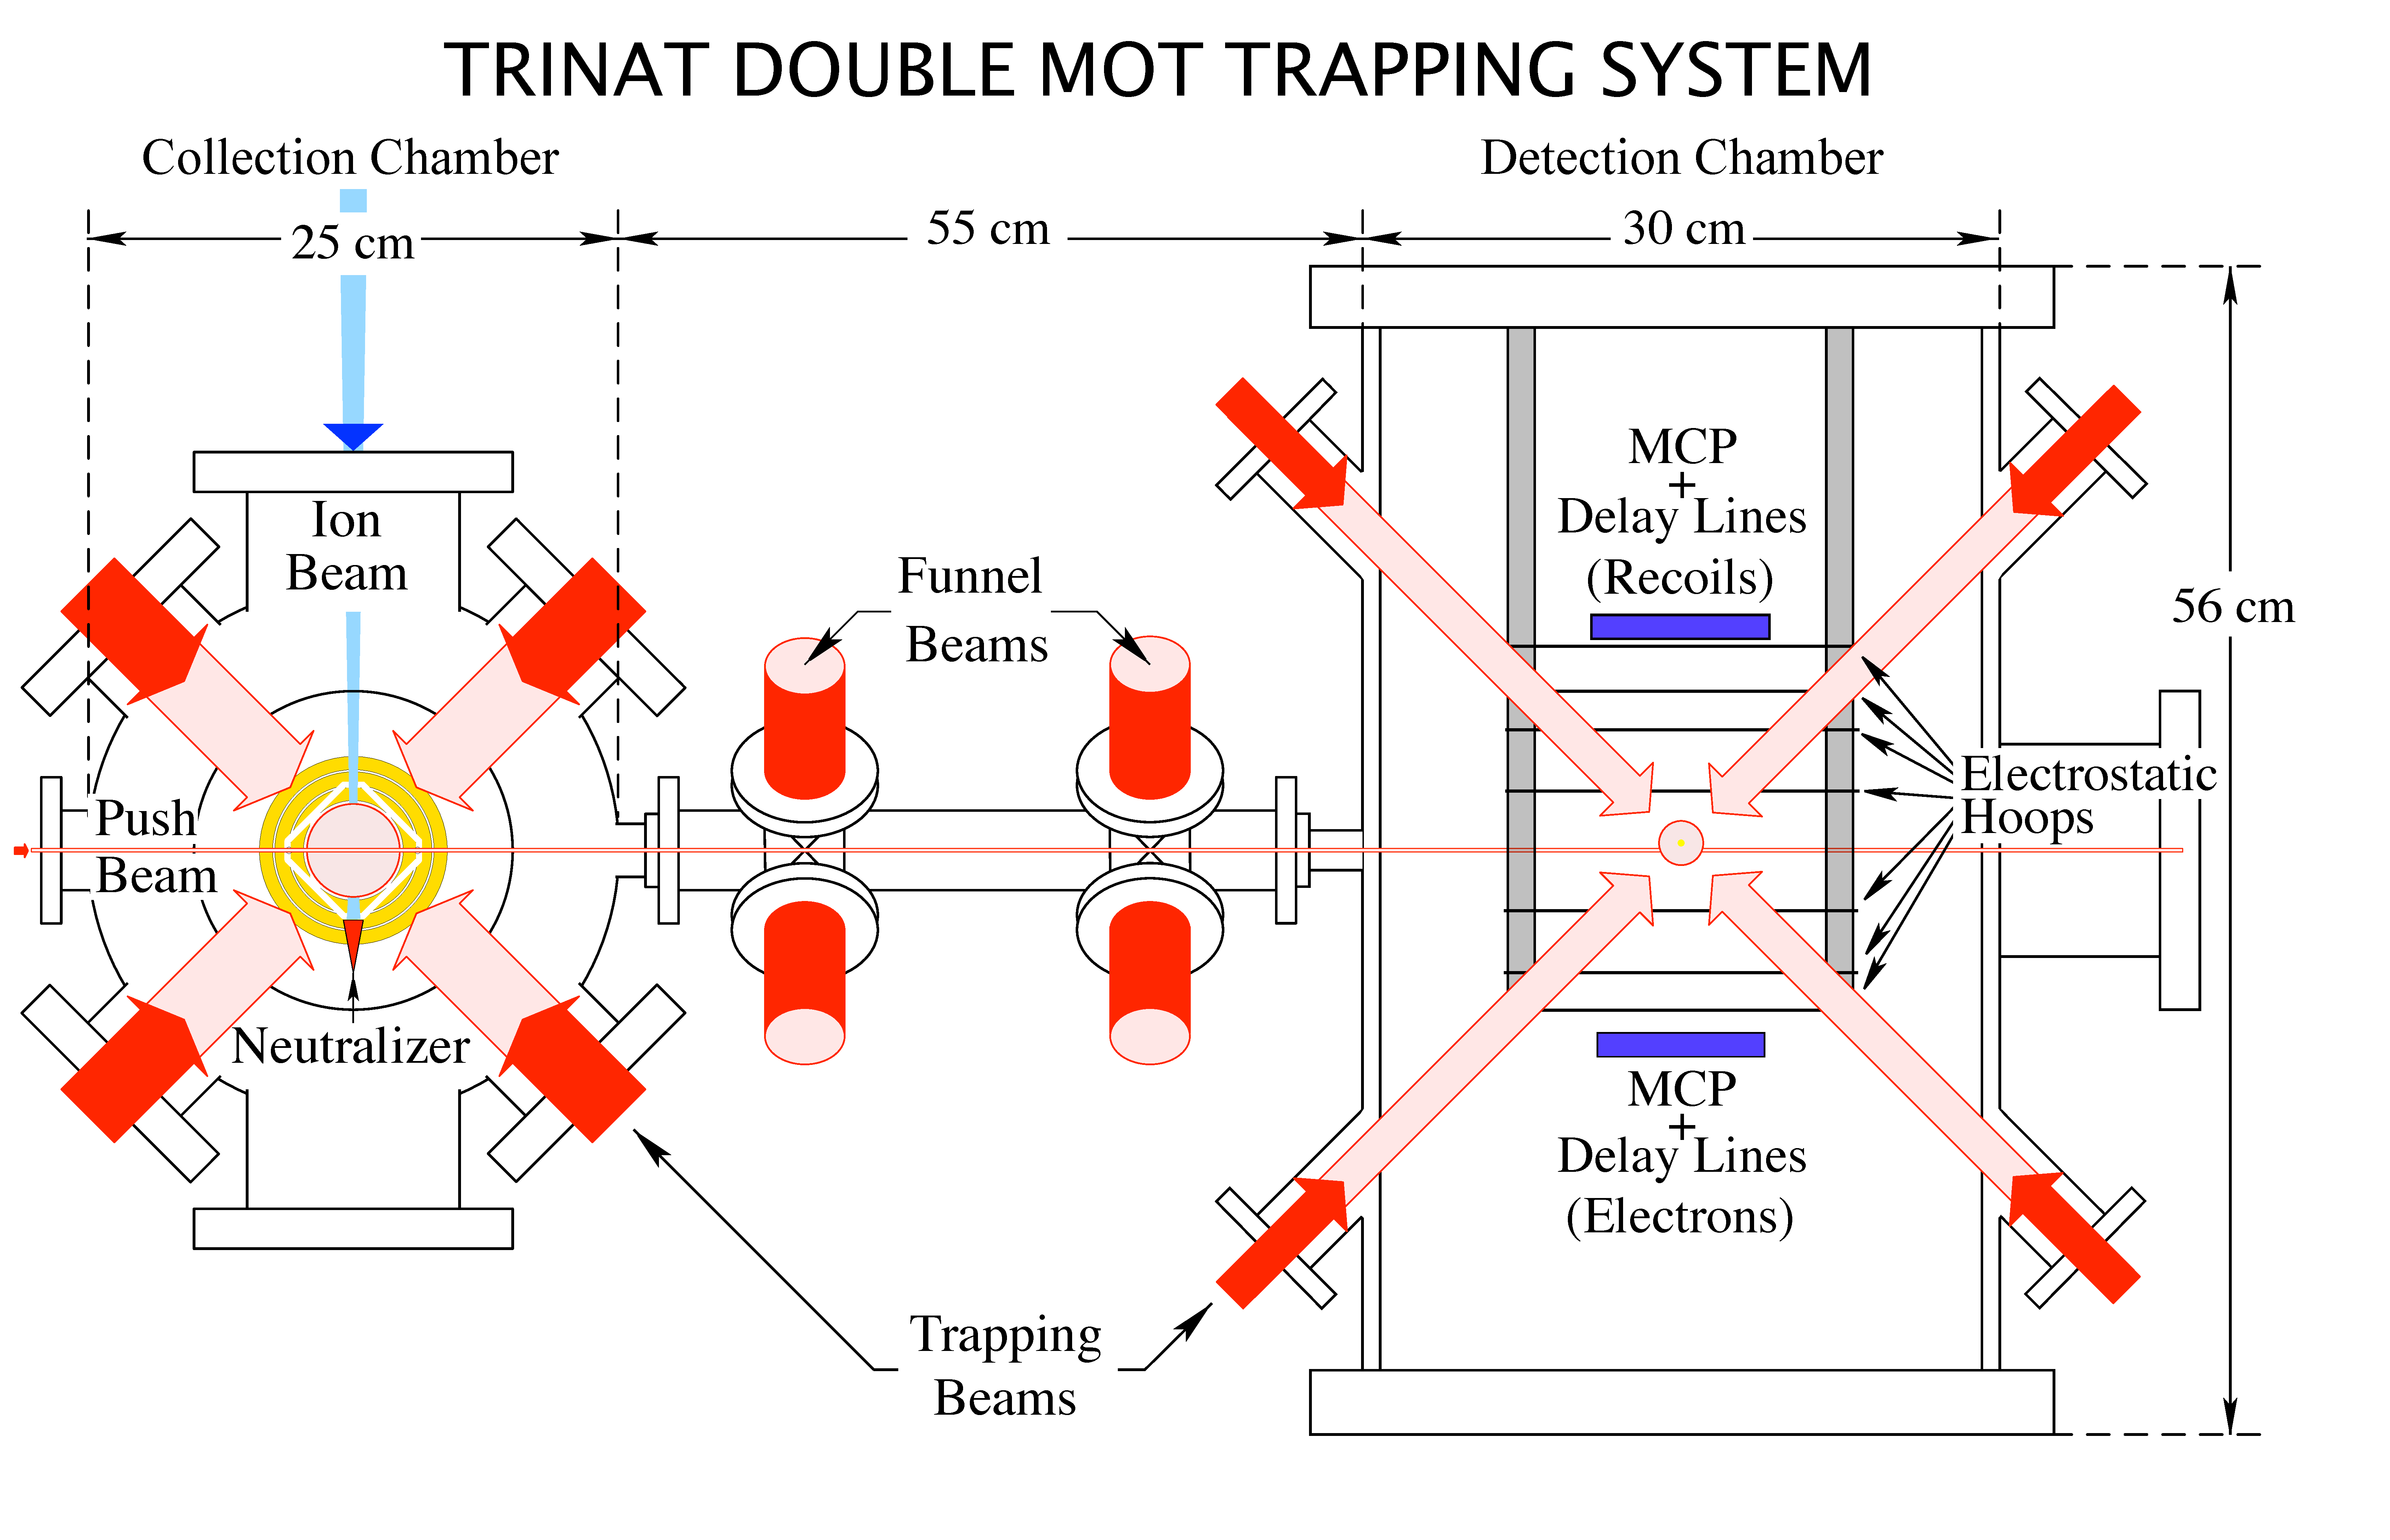
\includegraphics[width=.999\linewidth]
	{Figures/doublemot4.pdf}
	\caption{The TRINAT experimental set-up, viewed from above.  The two MOT system reduces background in the detection chamber.  Funnel beams along the atom transfer path keep the atoms focused.}	
	\label{fig:doublemot}
\note{Figure was originally created by Alexandre, modified by ... someone else?  Or Alexandre?  And I got it from ... probably an experimental proposal?}
\end{figure}

The TRINAT lab accepts radioactive ions delivered by the ISAC beamline at TRIUMF.  These ions are collected on the surface of a hot zirconium foil where they are electrically neutralized, and subsequently escape from the foil into the first of two experimental chambers (the ``collection chamber").  Further details on the neutralization process are presented in a previous publication~\cite{gorelov2000}.  Within the collection chamber, atoms of one specific isotope -- for the purposes of this thesis,  \isotope[37]{K} -- are continuously collected into a magneto-optical trap (MOT) from the tail end of the thermal distribution.  Although this procedure preferrentially traps only the slowest atoms, once trapped, atoms will be cooled further as a side-effect of the MOT's trapping mechanism.  The result is a small ($\sim\!1\,$mm diameter), cold ($\sim\!1\,$mK) cloud of atoms of a particular isotope.  

These properties allow for a relatively clean transfer of linear momentum from an appropriately tuned laser beam to the atoms within the cloud, and we use this mechanism to ``push'' the atoms out of the collection MOT and into the ``detection chamber'', where they are loaded into a second MOT (see Fig.~\ref{fig:doublemot}).  During regular operation, atoms are transferred approximately once per second.  It should be noted that this loading process does not require atoms already trapped within the second MOT to be released when a new set of atoms is loaded.    

Because the transfer and trapping mechanisms rely on tuning to specific atomic resonances, they act on only a single isotope.  The result is a significant reduction of background contaminants within the detection chamber, relative to the initial beamline output.  
%this setup allows for the selection of only a single isotope within the detection MOT, and a significantly reduced background relative to the initial beamline output.  
The transfer methodology is discussed in some detail within another publication~\cite{swanson}.

%\note{Probably describe the laser transfer method slightly.}  

%The TRIUMF Neutral Atom Trap (TRINAT) offers an experimental set-up which is uniquely suited to precision tests of Standard Model beta decay physics.  Radioactive ions are delivered from the ISAC beamline and neutralized before being trapped in the first of two magneto-optical traps (MOTs).  Approximately once per second, atoms from the first MOT are transferred to the second, where their decay products can be observed with significantly less background than would have been possible in the first trap (see Figure~\ref{fig:doublemot}).  The transfer methodology is discussed in some detail in a paper by Swanson et al~\cite{swanson}. \aside{The point is that this eliminates background from the decays of other stuff.  Or the same stuff.  Stuff that's not centered at the trap.}


Once the newly transferred atoms have arrived at the second trap, the MOT cycles 500 times between a state where it is `on' and actively confining atoms to a region of approximately 2\,mm$^3$, to a state where it is `off' and instead the atoms are spin-polarized by optical pumping while the atom cloud expands ballistically before being re-trapped.  Immediately following each set of 500 optical pumping cycles, another set of atoms is transferred in from the collection chamber to the detection chamber, joining the atoms that remain in the trap.  See Fig.~\ref{fig:dutycycle}.  This details of the trapping and optical pumping cycles are described further in Section~\ref{section:acmot_and_polarization}, and the optical pumping technique and its results are the subject of a recent publication~\cite{ben_OP}.

\begin{figure}[h!!t]
	\centering
	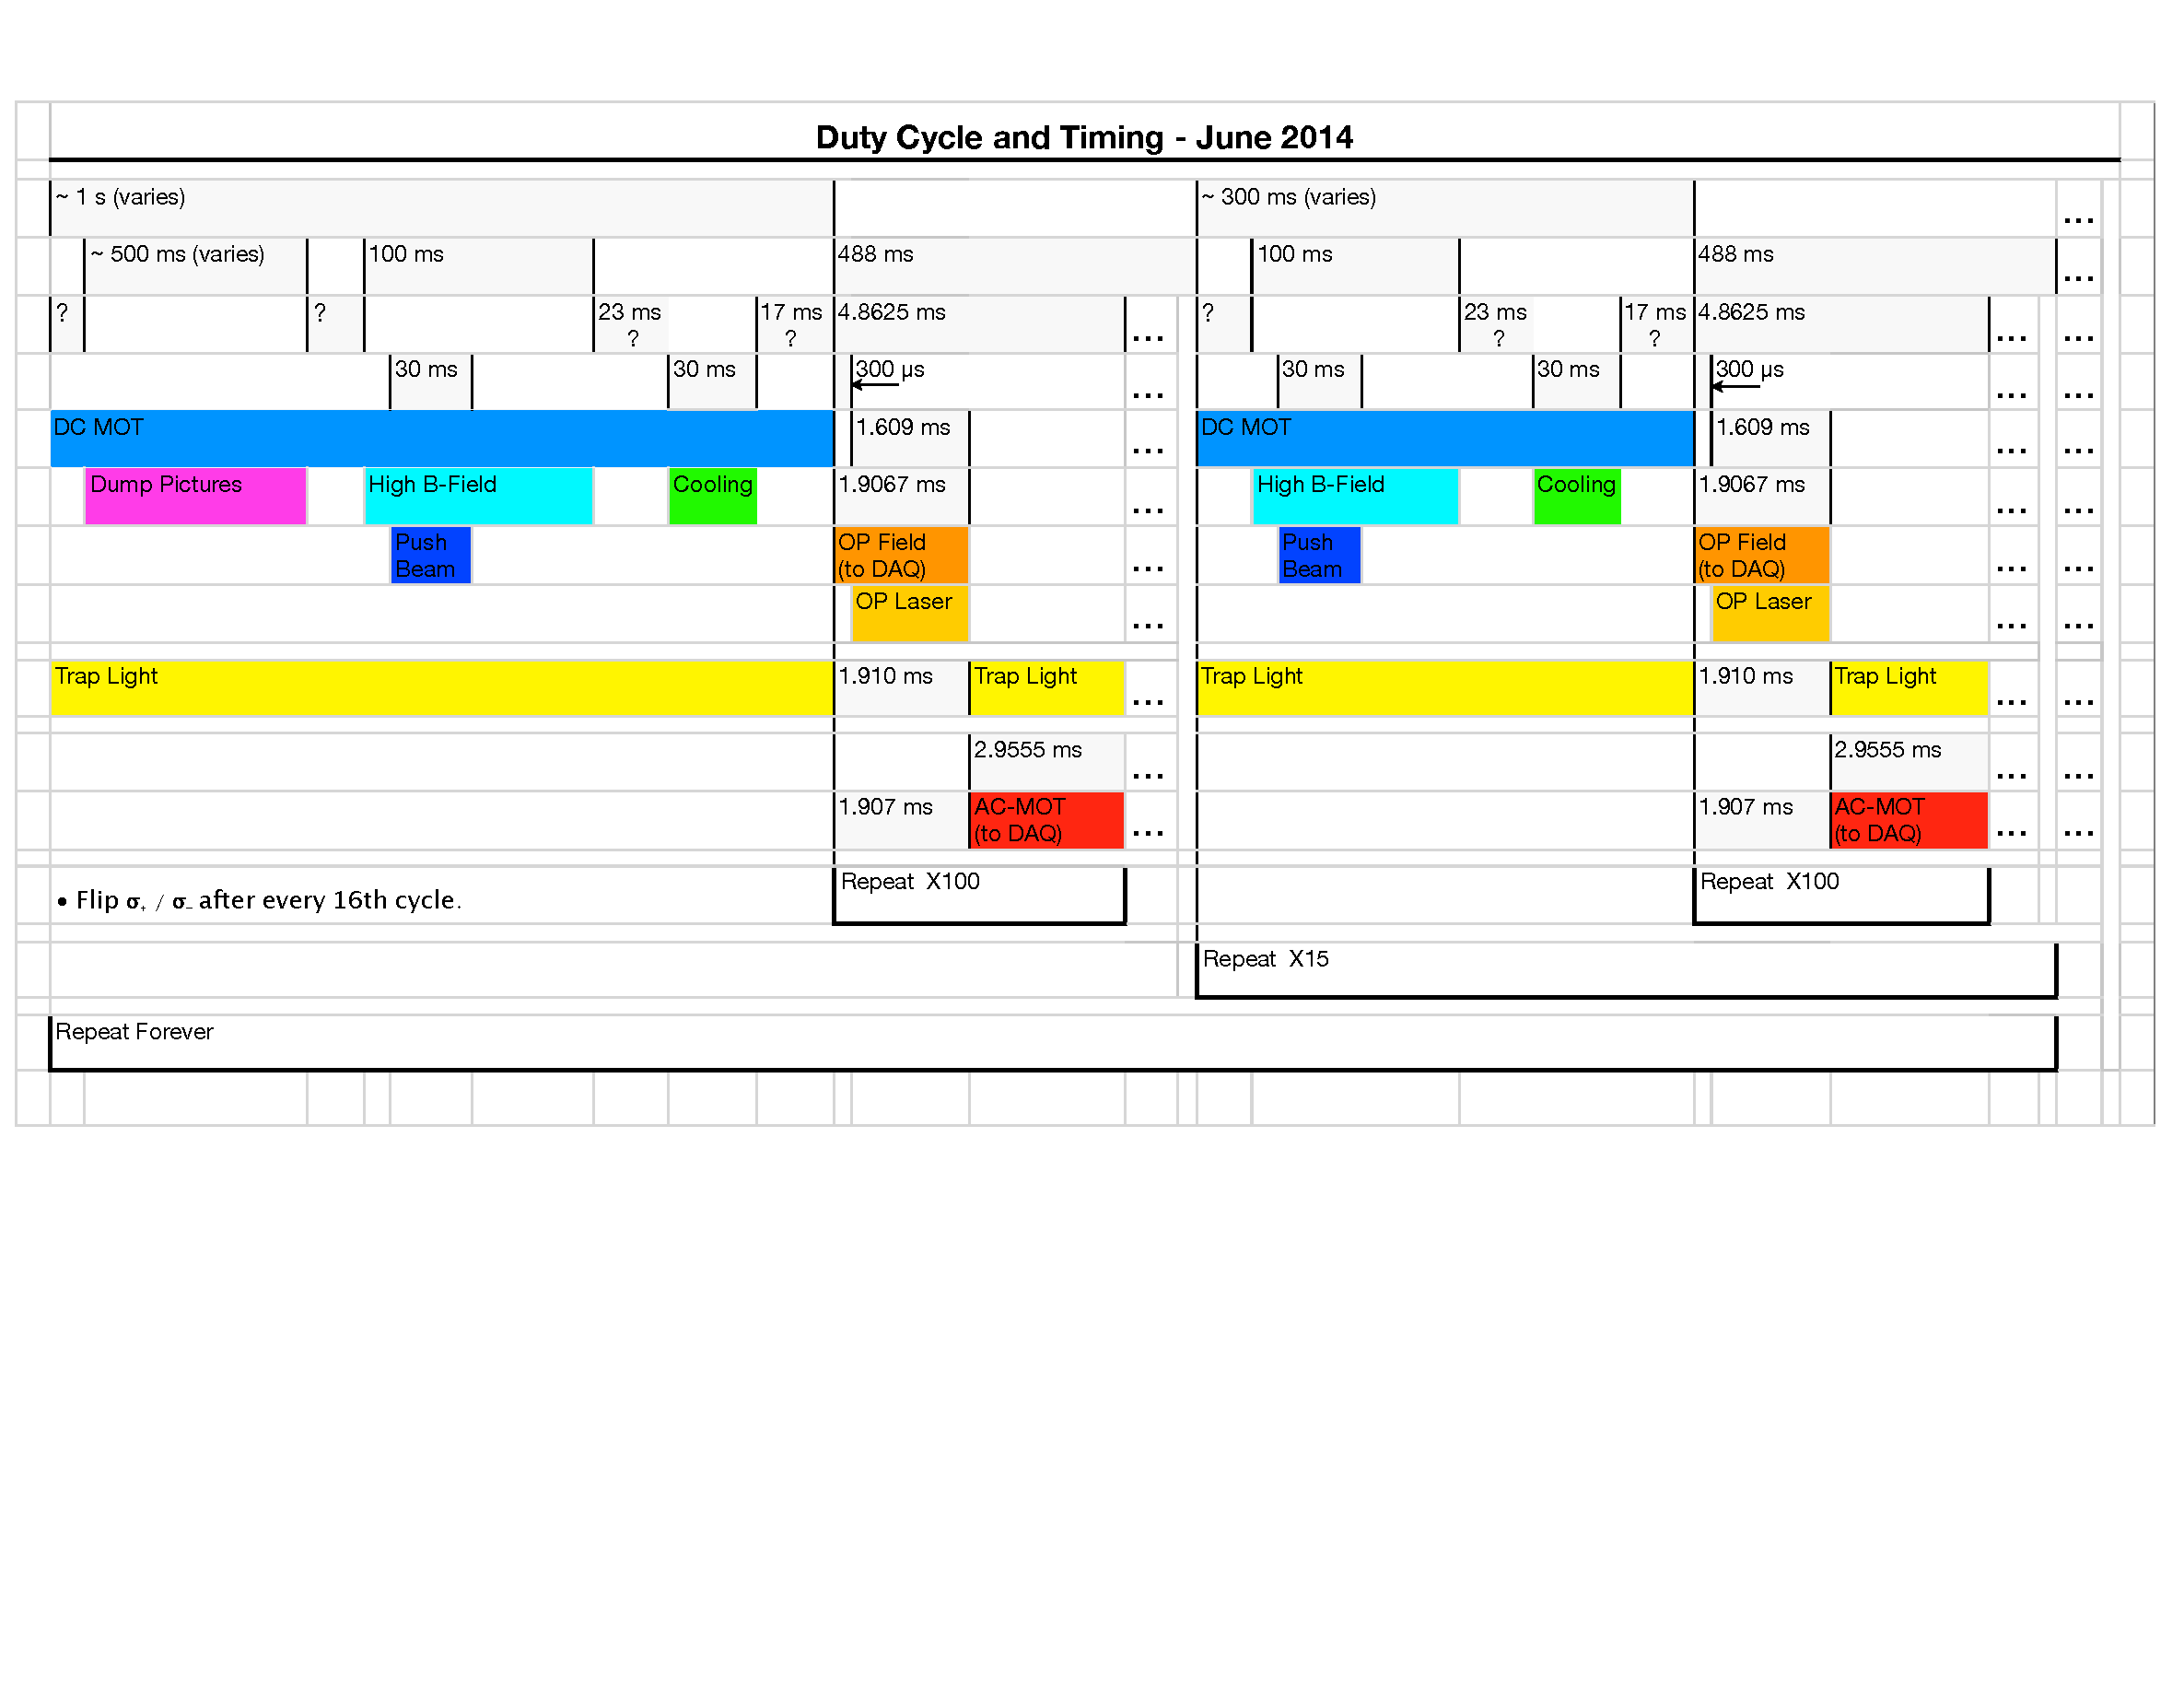
\includegraphics[width=.999\linewidth]
	{Figures/DutyCycle_2014.pdf}
	\caption{The duty cycle used for transferring, cooling, trapping, and optically pumping $\isotope[37]{K}$ during the June 2014 experiment.}	
	\label{fig:dutycycle}
\end{figure}
\note{Mumble mumble UHV.  Mumble mumble tail end of the Boltzmann distribution.}

\section{The AC-MOT and Polarization Setup}
\label{section:acmot_and_polarization}
%\\*
In order to facilitate a measurement of $A_{\mathrm{\beta}}$, great efforts were taken to polarize the atom cloud, and to quantify that polarization.  
%This resulted in a duty cycle in which the atoms were intermittently trapped in the AC-MOT, then optically pumped to polarize them.  
While knowledge of the polarization is arguably less critical to a measurement of $b_{\mathrm{Fierz}}$, it can still be a great asset, primarily for eliminating systematic effects.  We use only the polarized portion of the duty cycle in order to minimize other systematic errors, such as the scintillator energy calibration and overall trap position.  \note{What else does polarization get us?  The superratio, mostly.  Plus, it barely makes sense to measure $bFierz$ if you don't know $\Abeta$.}

\note{In order to eliminate systematic effects, the polarization direction is flipped every 16 seconds.}

\note{Probably document things about the waveform and frequency used for the beamtime, since I don't think it's in my MSc.}

The Magneto-Optical Trap is a well-known technique from atomic physics, used to confine and cool neutral atoms~\cite{raabprentiss}.  The technique is used predominantly with alkalis due to their simple orbital electron structure, and is quite robust, so is appropriate for use with $^{37}\textrm{K}$.  Once set up, the trapping force is specific to the isotope for which the trap has been tuned, which makes it ideal for use in radioactive decay experiments, since the daughters are unaffected by the trapping forces keeping the parent confined.

There are two primary components necessary for any MOT:  a laser, and a magnetic field.  The laser, which must be circularly polarized in the appropriate directions and tuned slightly to the red of an atomic resonance, is split into three perpendicular retroreflected beams, doppler cooling the atoms and (with the appropriate magnetic field) confining them in all three dimensions (see Figure~\ref{fig:mot}).  The TRINAT science chamber includes 6 `viewports' specifically designed to be used for the trapping laser.

\missingfigure{This is going to need another edge-on G4 picture of the chamber to label all the atomic components.  }

\missingfigure{I need \emph{at least} one atomic level diagram.  But possibly as many as 3 level diagrams.  Have to show energies for MOT, energies for OP, and energies for photoionization.  }
\note[color=purple]{JB says:  ``I would say you don't need an atomic level diagram.  You could just describe in words the semiclassical picture of atoms absorbing photons until they are nearly fully polarized, then they stop absorbing.  The optical pulmping + photoionization is then an in situ probe of the polarization. ... You would need to add in words that quantum mechanical corrections to this picture are in the optical Bloch equation approach in B. Fenker et al.  The depolarized states still have high nuclear polarization (1/2 for $F=2, M_F=1$, 5/6 for $F=1, M_F=1$) and determining the ratio of those two populations provides most of the info we need -- we model with the O.B.E, measure the optical pumping light polarization, and float an average transverse magnetic field.  This is adequate to determine the depolarized fraction to 10\% accuracy, which is all that is needed.'' }

\[\]

\note{Is my photoionization description adequate?  ... in light of John's feedback:  no.}
\note[color=jb]{JB says:  ``Since you worked hard on the logic triggers, a photoion spectrum with duty cycle would be appropriate if you want."}

\note{Need to describe how polarization works.}
\note[color=jb]{JB says:  all polarization details could be deferred to ~\cite{ben_OP}.  (be sure to list all authors including [me]).  )}


A MOT also requires a quadrupolar magnetic field, which we generate with two current-carrying anti-Helmholtz coils located within the vacuum chamber itself.  The coils themselves are hollow, and are cooled continuously by pumping temperature-controlled water through them.   

One feature which makes our MOT unusual has been developed as a result of our need to rapidly cycle the MOT on and off -- that is, it is an ``AC-MOT''.  Rather than running the trap with one particular magnetic field and one set of laser polarizations to match, we run a sinusoidal AC current in the magnetic field coils, and so the sign and magnitude of the magnetic field alternate smoothly between two extrema, and the trapping laser polarizations are rapidly swapped to remain in sync with the field~\cite{harveymurray}\cite{thesis}.  See Figure~\ref{fig:acmot}.  

\note{Note that because the atoms within a MOT can be treated as following a thermal distribution, some fraction of the fastest atoms continuously escape from the trap's potential well.  Even with the most carefully-tuned apparatus, the AC-MOT cannot quite match a similar standard MOT in terms of retaining atoms.  The TRINAT AC-MOT has a `trapping half-life' of around 6 seconds, and although that may not be particularly impressive by the standards of other MOTs, it is more than adequate for our purposes.  $^{37}\textrm{K}$ itself has a radioactive half-life of only 1.6 seconds 
(cite someone), so our dominant loss mechanism is radioactive decay rather than thermal escape. }



\note[color=green]{Anyway, here's some figures.  Or possibly one figure.  Whatever.  Also, here's a reference to a figure.  See Fig.~\ref*{fig:themot} (works -- currently ``3.4"), or also its subfigures, eg Fig.~\ref{fig:acmot} (works -- currently ``3.4b") and Fig.~\ref{fig:mot} (works -- currently ``3.4a").  Maybe I have to subref them?  Like, eg, Subfig.~\subref{fig:acmot} (works -- currently ``3.4b") and Subfig.~\subref*{fig:mot} (works -- currently ``3.4a").  What if we try to subref everything?  Consider, eg, Fig.~\subref{fig:themot} (doesn't work).  Yeah, ok, so fortunately the note cites like the text.  This gives an example of shit to do and not to do.  Also, can't do a linebreak within a note.}  

% !TEX root = ../thesis_main.tex

% fig:themot
% 	fig:mot
% 	fig:acmot

\begin{figure}[ht]
	\centering
	\begin{subfigure}[t]{0.242\textwidth}
		\centering
		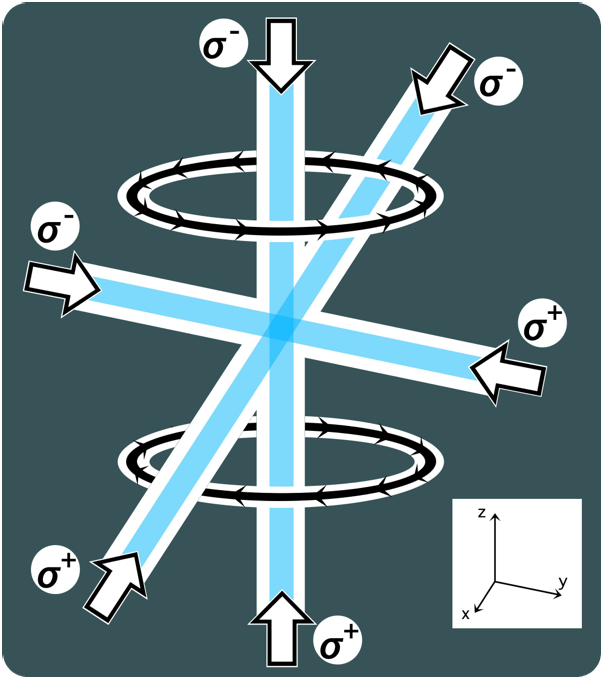
\includegraphics[width=\textwidth]{mot.png}
		\caption{Components of a magneto-optical trap, including current-carrying magnetic field coils and counterpropagating circularly polarized laser beams.}
		\label{fig:mot}
	\end{subfigure}
	\hfill
	\begin{subfigure}[t]{0.728\textwidth}
		\centering
		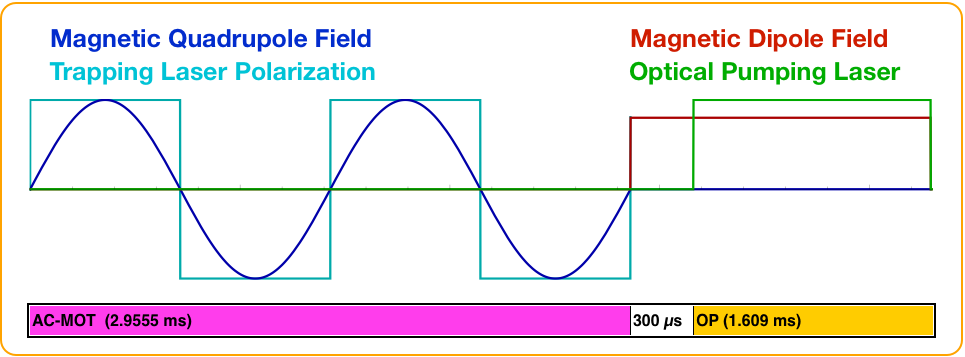
\includegraphics[width=\textwidth]{acmot.png}
		\caption{One cycle of trapping with the AC-MOT, followed by optical pumping to spin-polarize the atoms.  After atoms are transferred into the science chamber, this cycle is repeated 500 times before the next transfer.  The magnetic dipole field is created by running parallel (rather than anti-parallel as is needed for the MOT) currents through the two coils.}
		\label{fig:acmot}
	\end{subfigure}
	\caption{An alternating-current magneto-optical trap with a duty cycle optimized for producing polarized atoms}	
	\label{fig:themot}
\end{figure}

% fig:themot
% 	fig:mot
% 	fig:acmot



We spin-polarize $^{37}\textrm{K}$ atoms within the trapping region by optical pumping~\cite{ben_OP}.  A circularly polarized laser is tuned to match the relevant atomic resonances, and is directed through the trapping region along the vertical axis in both directions.  When a photon is absorbed by an atom, the atom transitions to an excited state and its total angular momentum (electron spin + orbital + nuclear spin) along the vertical axis is incremented by one unit.  When the atom is de-excited a photon is emitted isotropically, 
%\comment{(is it still isotropic when it's polarized?  I bet it's not.)}
so it follows that if there are available states of higher and lower angular momentum, the \emph{average} change in the angular momentum projection is zero.  If the atom is not yet spin-polarized, it can absorb and re-emit another photon, following a biased random walk towards complete polarization.  

%\missingfigure{Need a picture of the whole duty cycle.  Possibly combine with ~\ref{fig:acmot}.}


In order to optimally polarize a sample of atoms by this method, it is necessary to have precise control over the magnetic field.  This is because absent other forces, a spin will undergo Larmor precession about the magnetic field lines.  In particular, the magnetic field must be aligned along the polarization axis (otherwise the tendency will be to actually depolarize the atoms), and it must be uniform in magnitude over the region of interest (otherwise its divergencelessness will result in the field also having a non-uniform direction, which results in a spatially-dependent depolarization mechanism).  Note that this type of magnetic field is not compatible with the MOT, which requires a linear magnetic field gradient in all directions (characteristic of a quadrupolar field shape), and has necessitated our use of the AC-MOT as described in Section~\ref{section:acmot_and_polarization}.\aside{that's this section.  I should really describe the AC-MOT.}



\section{Microchannel Plates and Electric Field}
\label{section:mcps}
MCPs.  Hoops.  Only one thing works at a time!  Blarg.  Upon decay, atoms literally aren't trapped anymore by the trap.  No trapping forces, no slowing forces, because it's all isotope-specific.
\missingfigure{Back-to-back MCPs in an electric field to tag events from the trap, and to measure the trap position and polarization.  Hoops to produce the electric field.}

%\color{black}
%	\subsection{\textbf{Nuclear Setup}}
\section{Measurement Geometry and Detectors}
\label{section:betadetectors}
\note{This section is disorganized and repeats itself.}
\comment{
%\note{Do I want to make an entirely new section for the MCPs and electric field stuff?  It doesn't seem to quite fit in either of the two sections here...}
	Needs several diagrams.  %Back-to-back beta detectors along the polarization axis.  Back-to-back MCPs in an electric field to tag events from the trap, and to measure the trap position and polarization.  Hoops to produce the electric field.  
	Many laser ports to make the MOT functional, and for optical pumping.  Fancy mirror geometry to combine optical pumping and trapping light along the vertical axis.  Water-cooled (anti-)Helmholz coils within the chamber for the AC-MOT, fast switching to produce an optical pumping field.  
%	\subsection{\textbf{All the Detectors}}
}

% !TEX root = ../thesis_main.tex


% "fig:thechamber"

\begin{figure}[h!!!tb]
	\centering
%	\hspace*{\fill}%
	\subfloat[A decay event within the TRINAT science chamber.  After a decay, the daughter will be unaffected by forces from the MOT.  Positively charged recoils and negatively charged shake-off electrons are pulled towards detectors in opposite directions.  Although the $\beta^+$ is charged, it is also highly relativistic and escapes the electric field with minimal perturbation.
	%\comment{The pic is still kind-of fuzzy.}
	]
	{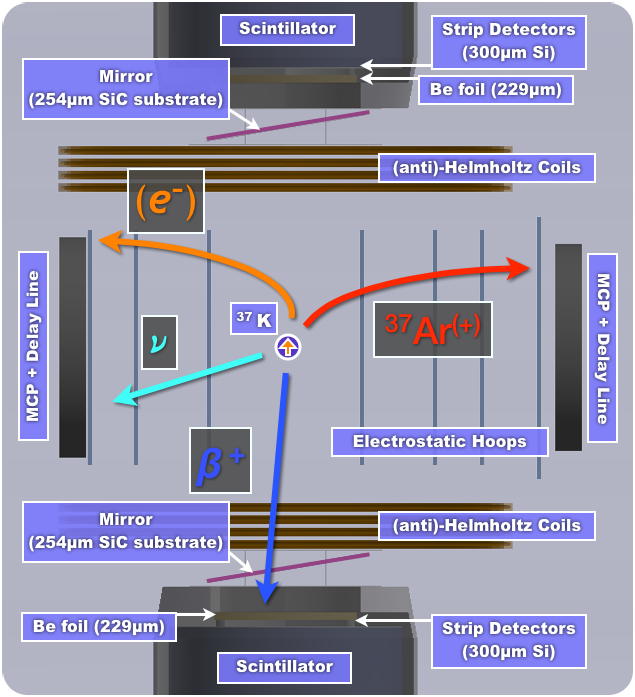
\includegraphics[width=.530\linewidth]{Figures/chamber_decayevent3.png}\label{chamber_decayevent} }
	\hspace*{\fill}
%	\hfill
	\hspace*{\fill}
	\subfloat[Inside the TRINAT science chamber.  This photo is taken from the vantage point of one of the microchannel plates, looking into the chamber towards the second microchannel plate.  The current-carrying copper Helmholtz coils and two beta telescopes are visible at the top and bottom.  The metallic piece near the center is one of the electrostatic `hoops' used to generate an electric field within the chamber.  The hoop's central circular hole allows access to the microchannel plate, and the two elongated holes on the sides allow the MOT's trapping lasers to pass unimpeded at an angle of 45 degress `out of the page'.]	
	{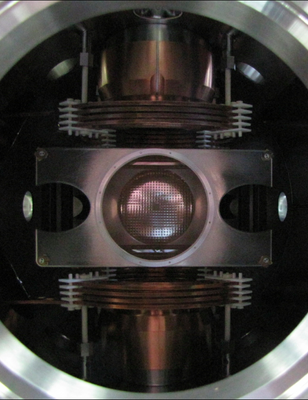
\includegraphics[width=.444\linewidth]{Figures/chamber_photo_2.png}}
%	\hspace*{\fill}%
	\caption{The TRINAT detection chamber}	
	\label{fig:thechamber}
\end{figure}


% "fig:thechamber"

%\note{Below is pretty vague.  I could do better, even for just an overview-summary thing.  Obvs I have to describe it in detail later on *somewhere*, though maybe not in the overview-summary...} 
Detectors are positioned about the second MOT for data collection.  The detection chamber 
%(shown in Figure \ref{fig:thechamber}) 
operates at ultra-high vacuum (UHV) and provides not only the apparatus necessary to intermittently confine and then spin-polarize atoms, but also the variety of detectors and implements required to quantify their position, temperature, and polarization.  The detection chamber further boasts an array of electrostatic hoops to collect both positively and negatively charged low energy particles into two microchannel plates (MCPs),  and a further set of two beta detectors positioned along the polarization axis, each of which consists of a 40x40 pixel double-sided silicon strip detector (DSSD) and a scintillator and photomultiplier tube (PMT).  %The details of the detection chamber setup are described in detail in Section~\ref{section:betadetectors}. 
%\note{ ...where I basically repeat this same content.  Blarg.}




\note{...(shown in Figure \ref{fig:thechamber}) ...}
The beta detectors, located above and below the atom cloud along the axis of polarization (see Figure~\ref{chamber_decayevent}), are each the combination of a plastic scintillator and a set of silicon strip detectors.  Using all of the available information, these detectors are able to reconstruct the energy of an incident beta, as well as its hit position, and provide a timestamp for the hit's arrival.  Together the upper and lower beta detectors subtend approximately 1.4\% of the total solid angle as measured with respect to the cloud position. 

%\section{Beta Detectors}
	The two sets of beta detectors were positioned directly along the axis of polarization.  Each beta detector consists of a plastic scintillator and photo-multiplier tube (PMT) \aside{There's gotta be a better way to describe it} placed directly behind a 40$\times$40-pixel double-sided silicon strip detector (DSSD).  \aside{what's the open area of the detector?  how big is each pixel?}  The scintillator is used to measure the overall energy of the incoming particles, as well as to assign a timestamp to these events, while the DSSD is used both to localize the hit position to one (or in some cases, two) individual pixel(s), and also to discriminate between different types of incoming particles.  In particular, though the scintillator will measure the energy of an incoming beta or an incoming gamma with similar efficiency, the beta will lose a portion of its kinetic energy as it passes through the DSSD into the scintillator.  By contrast, an incident gamma will deposit only a very small amount of energy in the DSSD layer, making it possible to reject events with insufficient energy deposited in the DSSD as likely gamma ray events.  Given that the decay of interest to us emits positrons, we expect a persistent background 511 keV gamma rays that are not of interest to us, so it is extremely important that we are able to clean these background events from our spectrum. 


It must be noted that the path between the cloud of trapped atoms and either beta detector is blocked by two objects:  a 275$\,\mu$m silicon carbide mirror (necessary for both trapping and optical pumping), and a 229$\,\mu$m beryllium foil (separating the UHV vacuum within the chamber from the outside world).  In order to minimize beta scattering and energy attenuation, these objects have had their materials selected to use the lightest nuclei with the desired material properties, and have been manufactured to be as thin as possible without compromising the experiment.  As the $^{37}\textrm{K} \rightarrow \,^{37}\textrm{\!Ar} + \beta^{+} + \nu_e$ decay proceess releases $Q=5.125$\,MeV of kinetic energy~\cite{Q_value}, the great majority of betas are energetic enough to punch through both obstacles without significant energy loss before being collected by the beta detectors.  

On opposing sides of the chamber, and perpendicular to the axis of polarization, two stacks of $\sim$ 80\,mm diameter microchannel plates (MCPs) have been placed (see Figure~\ref{fig:thechamber}) as detectors, providing a time stamp when a particle is incident on their surfaces.  Behind each stack of MCPs there is a set of delay lines, which provide  position sensitivity for these detectors.   

In order to make best use of these MCPs, we create an electric field in order to draw positively charged particles into one MCP, while drawing negatively charged electrons into the other MCP.  Seven electrostatic hoops have been placed within the chamber (see Figure~\ref{fig:thechamber}), and are connected to a series of high voltage power supplies.  See Sections~\ref{photoions} and~\ref{pos_recoils} for a discussion of what sort of charged particles we expect to observe in these detectors and how they are created.  
  
Scientific data has been collected at field strengths of 395 V/cm, 415 V/cm, and 535 V/cm.  It should be noted that these field strengths are too low to significantly perturb any but the least energetic of the (positively charged) betas from the decay process, and these low energy betas would already have been unable to reach the upper and lower beta detectors due to interactions with materials in the SiC mirror and Be foil vacuum seal.  

